\documentclass{article}
\usepackage[german]{babel}
\usepackage{graphicx,hyperref,xcolor}

%%%%%%%%%% Start TeXmacs macros
%\catcode`\>=\active \def>{\fontencoding{T1}\selectfont\symbol{62}\fontencoding{\encodingdefault}}
\newcommand{\tmem}[1]{{\em #1}}
\newcommand{\tminput}[2]{\trivlist{\item[\color{rgb:black,10;red,9;green,4;yellow,2}{#1}]{\color{blue!50!black}\mbox{}#2}}}
\newcommand{\tmoutput}[1]{#1}
\newcommand{\tmsession}[3]{{\tt#3}}
\newcommand{\tmstrong}[1]{\textbf{#1}}
\newcommand{\tmunfoldedio}[3]{\trivlist{\item[\color{rgb:black,10;red,9;green,4;yellow,2}{#1}]\mbox{}{\color{blue!50!black}#2}\item[]\mbox{}#3}}
%%%%%%%%%% End TeXmacs macros

\begin{document}

{\tmstrong{Computational NLD}} Vorlesung 1 12.04.2016

{\tmstrong{}}{\tmstrong{Aufgabe 1 logitische Funktion in C++ programmieren}}

{\tmstrong{Aufgabe 1.1 logistische Funktion mit beliebigen Anfangswert
plotten}}

Das Programm .ccp erzeugt f{\"u}r ein beliebiges r und Startwert x ein
Diagramm

Parameter

\

\tmsession{shell}{default}{
  \tmoutput{Shell session inside TeXmacs pid = 8426}
  \tminput{Shell] }{g++ -o Vorl1-A1-1 Vorl1-A1-1.cpp \&\& ./Vorl1-A1-1 >
  V1-A1-1-E1.dat\\
  }
  \tminput{Shell] }{\ }
}

\tmsession{gnuplot}{default}{
  \tmunfoldedio{gnuplot] }{set xlabel 'Durchlauf i'; set ylabel 'x'; plot
  '{\tmem{}}V1-A1-1-E1.dat' with points pt 7 ps
  1}{\raisebox{0.0\height}{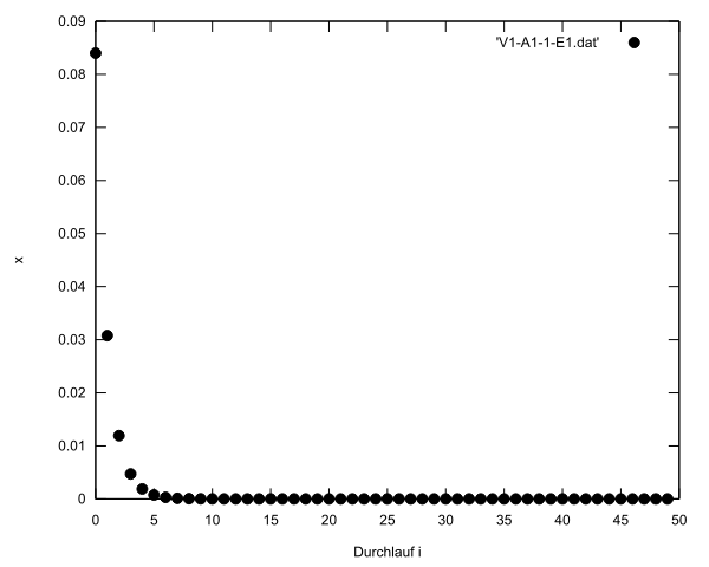
\includegraphics[width=11.89935064935065cm,height=9.519480519480519cm]{Vorlesung-1-1.pdf}}}
  \tminput{GNUplot] }{\ }
}

{\tmstrong{Aufgabe 1.2 \ logistische Funktion Bifurkationsdiagramm plotten
x-r-Diagramm}}

Das Programm \ erzeugt das Bifurkationsdiagramm f{\"u}r die logistische
Funktion

Parameter:

{\tmem{}}r = 0.1

x = 0.3blo

delta\_r = 0.01

\

\href{Vorl1-A2-1.cpp}{Vorl1-A2-1.cpp}

\tmsession{shell}{default}{
  \tmoutput{Shell session inside TeXmacs pid = 6021}
  \tminput{Shell] }{g++ -o Vorl1-A1-2 Vorl1-A1-2.cpp \&\& ./Vorl1-A1-2 >
  V1-A1-2-E1.dat}
  \tminput{Shell] }{\ }
}

\

\tmsession{gnuplot}{default}{
  \tmunfoldedio{GNUplot] }{set xlabel 'Parameter r'; set ylabel 'x'; plot
  '{\tmem{}}V1-A1-2-E1.dat' with points pt 7 ps
  0.5}{\raisebox{0.0\height}{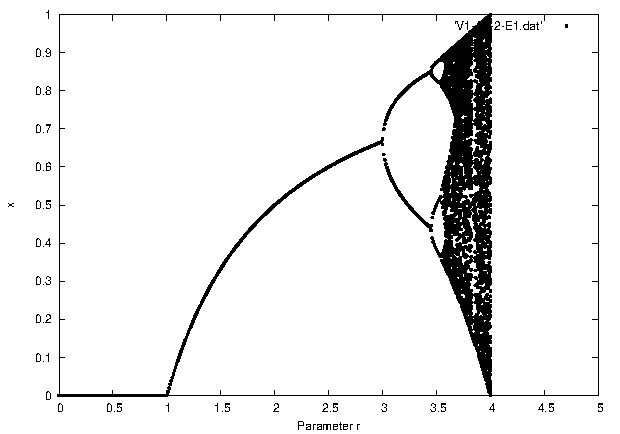
\includegraphics[width=10.411911321002231cm,height=7.288337924701561cm]{Vorlesung-1-2.pdf}}}
  \tminput{GNUplot] }{\ }
}

{\tmstrong{Aufgabe 2 Ikeda Map}}

\

\

\tmsession{gnuplot}{default}{
  \tmoutput{TeXmacs interface for GNUplot.}
  \tmunfoldedio{GNUplot] }{plot 'V1-A2-1-E1.dat' with points pt 7 ps 0.5\\
  }{\raisebox{0.0\height}{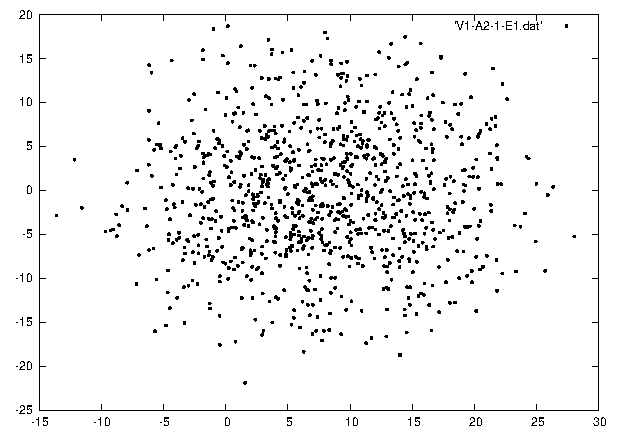
\includegraphics[width=10.411911321002231cm,height=7.288337924701561cm]{Vorlesung-1-3.pdf}}}
  \tminput{GNUplot] }{\ }
}

\end{document}
